\documentclass{article}
\usepackage{graphicx}
\usepackage{hyperref}

\begin{document}

\graphicspath{ {./Images/} }
\tableofcontents

\section{Introduction}
Hello and welcome to Windows. This document describes the process of configuring windows machines to run on Proxmox. If you would like to add something, please contribute in the github.

\section{Getting the correct ISOs to Proxmox}
The goal is to get both the Windows Server and the VirtIO driver iso files onto proxmox.

You should can either download the files to your computer and then to proxmox, or you can have proxmox download them from "download from url."

In either case, the Windows Server 2019 iso is \href{http://www.microsoft.com/en-us/evalcenter/download-windows-server-2019
}{here} and the VirtIO iso is \href{https://fedorapeople.org/groups/virt/virtio-win/direct-downloads/stable-virtio/}{here}.

The VirtIO is necessary because proxmox says so (update with better reasoning). \href{https://pve.proxmox.com/wiki/Windows_VirtIO_Drivers#Windows_OS_Support}

VirtIO also enables the QEMU Guest Agent, which allows for many convenient things in proxmox.

\begin{figure}[h]
    \centering
    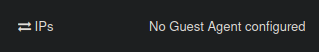
\includegraphics[width=0.5\textwidth]{noGuestAgent.png}
    \caption{The IP Address is not displayed if there is no guest agent}
    \label{fig:noGuestAgent}
\end{figure}

\section{Getting the VM}
Some guy doing it with no words: \href{https://www.youtube.com/watch?v=lwORpWEHiDE&t=5m}{video}

The important settings to click are:
OS -> Type: Microsoft Windows, Version: 10/2016/2019
System -> SCSI Controller: VirtIO SCSI Single, QEMU Agent checked
Disks -> Bus/Device: SCSI
Memory -> 4096 B of RAM
Cache to write-back cache

After creating this VM, click it and go to the “Hardware” menu in Proxmox. Click “add CD/DVD” and click the virtIO.iso file you uploaded.
\section{Modifying the VM}

\end{document}
